\chapter{Geräteverschlüsselung}
\section{Einleitung}
Die Verschlüsselung der Daten auf Geräten ist Teil der physischen Sicherheit.
Damit kann sichergestellt werden, dass keine Daten gestohlen werden können, wenn das Geräte verloren geht oder gestohlen wird.
Diese Sicherheit ist besonders wichtig, wenn Notebooks in der Firma eingesetzt werden.

\section{Verschlüsselung unter Windows}
In Windows gibt es zwei im \acrshort{os} integrierte Möglichkeiten, die Daten auf dem Gerät zu verschlüsseln.
In Windows Home gibt es die sogenannte ``Geräteverschlüsselung'' in den Systemeinstellungen.
Ab Windows Pro kann man Geräte mit ``BitLocker'' verschlüsseln.\\

\subsection{Windows Home Version}
In der Windows 10 Home Version gibt es die ``Geräteverschlüsselung''.
Da Windows 10 Home nicht für Unternehmen gedacht ist, gibt es auch keine Möglichkeit, die Geräteverschlüsselung zentral zu verwalten.
Sie muss auf jedem Gerät einzeln aktiviert werden.

Die ``Geräteverschlüsselung'' findet man unter \textbf{Settings $\rightarrow$ Update \& Security $\rightarrow$ Device encryption}

\subsection{Windows Pro/Enterprise Version}
Mit BitLocker kann man die Festplatten auf den Geräten schnell und einfach verschlüsseln.
Der Recovery Key wird im Computer Objekt in Active Directory hinterlegt.

\subsubsection{Voraussetzungen}
Um BitLocker unter Windows zu verwenden, wird ein \acrfull{tpm} Chip benötigt.
Falls das Gerät einen \acrshort{tpm} Chip hat, ist dieser im Gerätemanager unter ``Security Devices'' ersichtlich:
\begin{figure}[H]
    \centering
    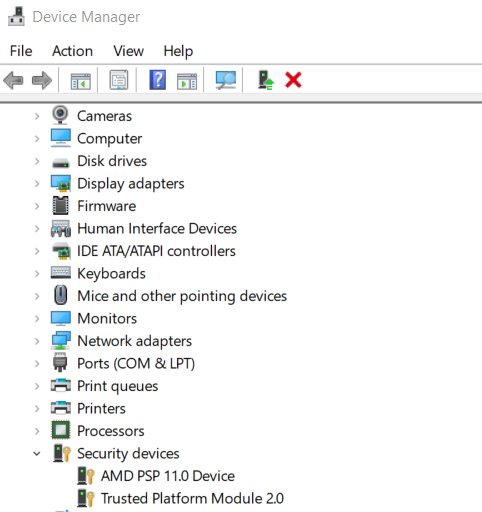
\includegraphics[width=0.6\linewidth]{../img/Encryption/tpm-chip-device-manager.png}
    \caption{\acrshort{tpm} Chip im Gerätemanager}
\end{figure}
Es gibt auch die Möglichkeit BitLocker ohne \acrshort{tpm} Chip zu verwenden. Dann muss jedoch bei jedem aufstarten ein Passwort eingegeben werden.

\subsubsection{BitLocker Feature}
Damit der Recovery Key in Active Directory hinterlegt wird, muss zuerst das BitLocker Feature auf dem Domain Controller aktiviert werden.
Dazu öffnet man den Server Manager, navigiert zu \textbf{Manage $\rightarrow$ Add Roles and Features}.
Unter ``Features'' wählt man ``Bitlocker Drive Encryption'' und installiert dieses Feature:
\begin{figure}[H]
    \centering
    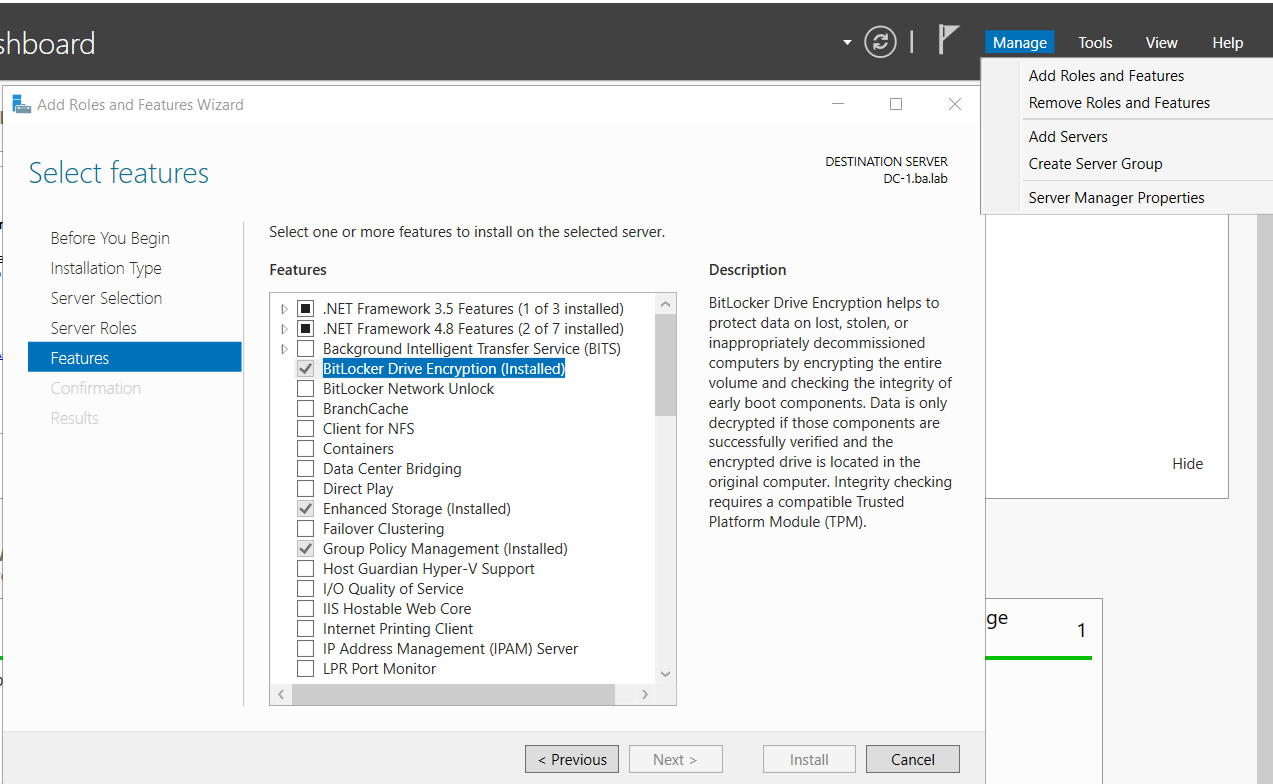
\includegraphics[width=0.7\linewidth]{../img/Encryption/bitlocker-feature.png}
    \caption{BitLocker Feature}
\end{figure}
\textbf{Wichtig:} Nach dem installiern muss der Server neugestartet werden.

\subsubsection{Group Policy}
Im Group Policy Management muss eine neue Group Policy erstellt werden, welche mit der \acrshort{ou} verknüpft ist, die die zu verschlüsselnden Windows Geräte enthält.
Mit \textbf{Rechtsklick $\rightarrow$ Edit} kann die neue Group Policy bearbeitet werden.
Unter \textbf{Computer Configuration $\rightarrow$ Policies $\rightarrow$ Administrative Templates $\rightarrow$ Windows Components $\rightarrow$ BitLocker Drive Encryption $\rightarrow$ Operating System Drives} kann mit \textbf{Rechtsklick $\rightarrow$ New $\rightarrow$ Package\dots} wird die Policy ``Choose how BitLocker-protected operating system drives can be recovered'' wie folgt eingerichtet:
\begin{figure}[H]
    \centering
    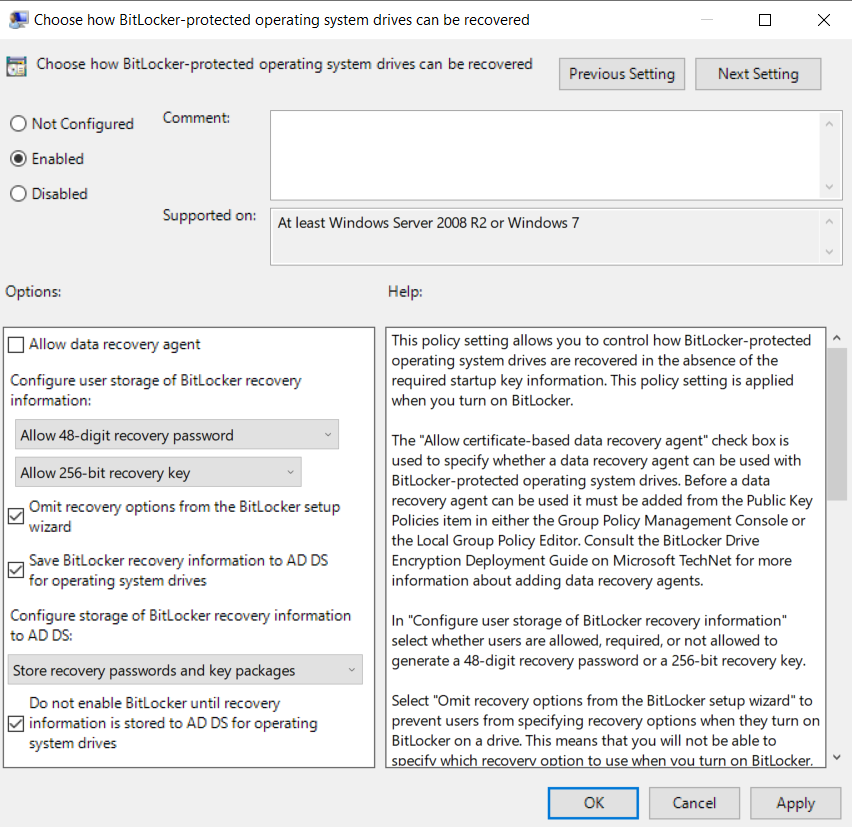
\includegraphics[width=0.7\linewidth]{../img/Encryption/store-bitlocker-in-ad.png}
    \caption{BitLocker Policy}
\end{figure}

Da Microsoft keinen zentralen Weg bietet, BitLocker auf den Geräten zu aktivieren, wird dies mit einem Script erledigt.
Dazu speichert man folgenden Powershell Code als .ps1 Datei ab:
\begin{lstlisting}
    $BitLockerVolume = Get-BitLockerVolume -MountPoint 'c:'
    if ($BitLockerVolume.VolumeStatus -eq 'FullyDecrypted') {
        Add-BitLockerKeyProtector -MountPoint 'c:' -RecoveryPasswordProtector
        Enable-Bitlocker -MountPoint 'c:' -TpmProtector
    }
\end{lstlisting}
Das Script muss auf einem freigegebenen Netzlaufwerk abgespeichert werden, auf welches alle Geräte Lesezugriff haben.
Zum Beispiel auf dem Domain Controller unter:
\begin{lstlisting}
    C:\Windows\SYSVOL\sysvol\<Domain>\scripts
\end{lstlisting}
\begin{figure}[H]
    \centering
    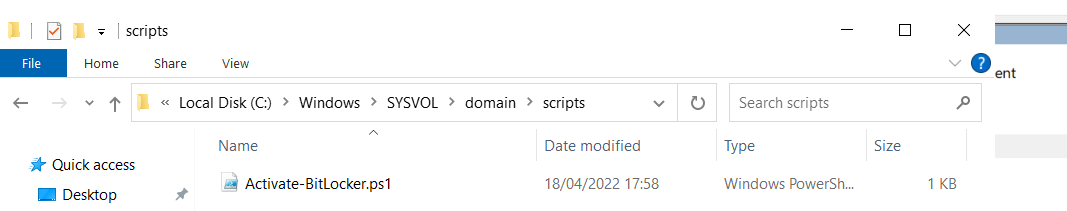
\includegraphics[width=\linewidth]{../img/Encryption/activate-bitlocker-script.png}
    \caption{BitLocker Scripts}
\end{figure}

Da die Installation mit einem Script gemacht wird, muss zuerst noch erlaubt werden, dass in Powershell Skripte ausgeführt werden dürfen.
Die Erlaubnis kann unter \textbf{Computer Configuration $\rightarrow$ Policies $\rightarrow$ Administrative Templates $\rightarrow$ Windows Components $\rightarrow$ Windows Powershell} mit der Policy ``Turn on Script Execution'' erteilt werden:
\begin{figure}[H]
    \centering
    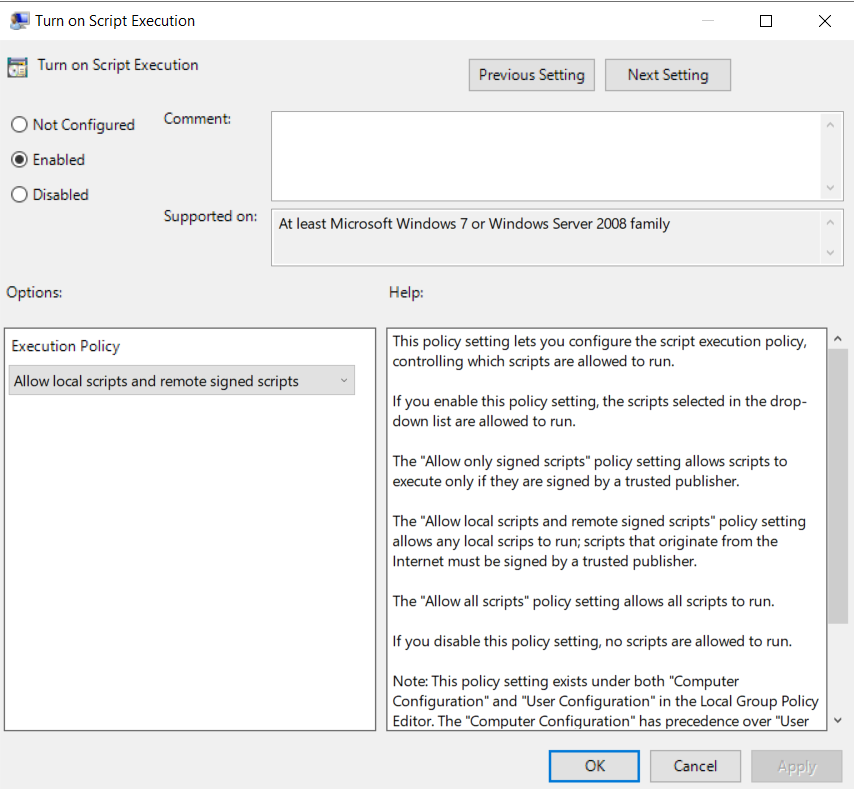
\includegraphics[width=\linewidth]{../img/Encryption/powershell-execution.png}
    \caption{Powershell Scripts aktivieren}
\end{figure}

Als nächstes muss unter \textbf{Computer Configuration $\rightarrow$ Preferences $\rightarrow$ Control Panel Settings $\rightarrow$ Scheduled Task} ein neuer ``Immediate Task (At least Windows 7)'' erstellt werden:
\begin{figure}[H]
    \centering
    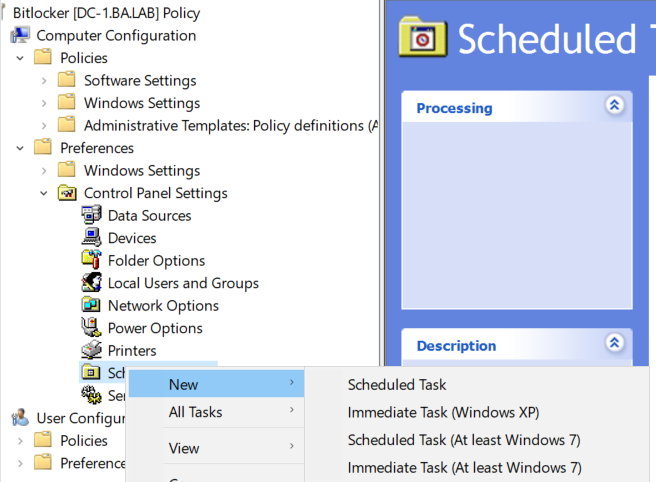
\includegraphics[width=0.7\linewidth]{../img/Encryption/new-scheduled-task.png}
    \caption{Neuer Scheduled Task für BitLocker}
\end{figure}

Beim Scheduled Task werden folgende Einstellungen getroffen:\\
\begin{minipage}{0.5\linewidth}
    \begin{figure}[H]
        \centering
        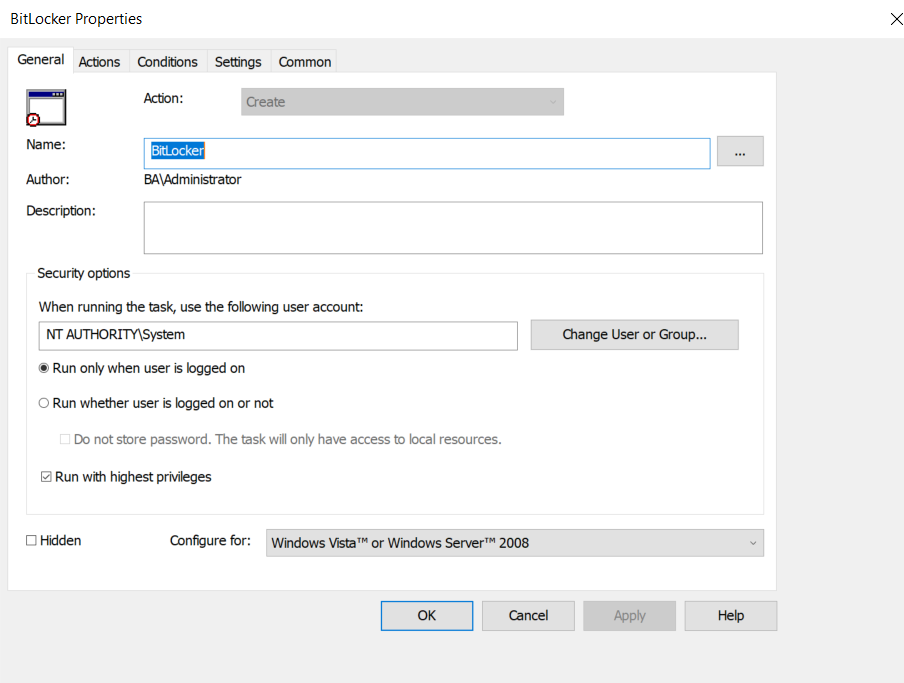
\includegraphics[width=\linewidth]{../img/Encryption/scheduled-task-1.png}
        \caption{Scheduled Task Einstellungen 1}
    \end{figure}
\end{minipage}
\begin{minipage}{0.5\linewidth}
    \begin{figure}[H]
        \centering
        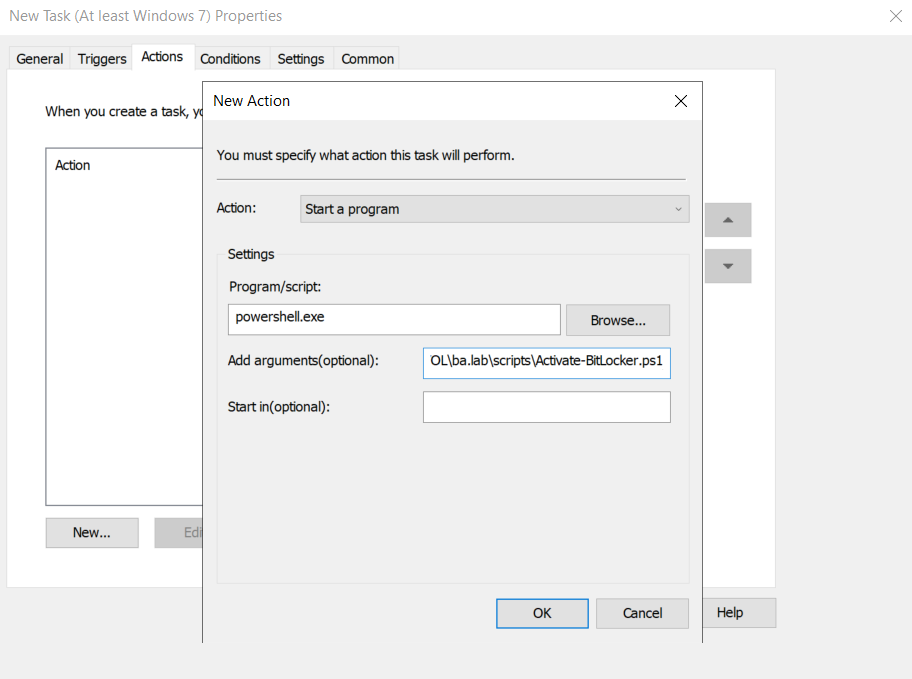
\includegraphics[width=\linewidth]{../img/Encryption/scheduled-task-2.png}
        \caption{Scheduled Task Einstellungen 2}
    \end{figure}
\end{minipage}\\

Bei ``Add Arguments'' in ``New Action'' wird der \textbf{freigegebene} Pfad vom .ps1 Script angegeben.\\
Zum Beispiel:
\begin{lstlisting}
    \\<Hostname DC>\SYSVOL\<Domäne>\scripts\Activate-BitLocker.ps1
\end{lstlisting}

Die Festplatte wird beim nächsten Neustart verschlüsselt.
Es wird nur die Festplatte mit dem Betriebssystem verschlüsselt.
Falls man weitere Festplatten verschlüsseln will, muss man den ``MountPoint'' Parameter im Script anpassen.

\paragraph{BitLocker ohne \acrshort{tpm}}
BitLocker kann wie erwähnt auch ohne \acrshort{tpm} Chip verwendet werden, dann muss jedoch ein Passwort gesetzt werden.
Wenn BitLocker so verwendet werden möchte, muss man noch eine zusätzliche Policy für diese Geräte aktivieren.
Die Policy befindet sich am gleichen Ort wie die vorherige Policy um BitLocker zu aktivieren und heisst ``Require additional authentication at startup''.
Dort setzt man folgende Einstellungen:
\begin{figure}[H]
    \centering
    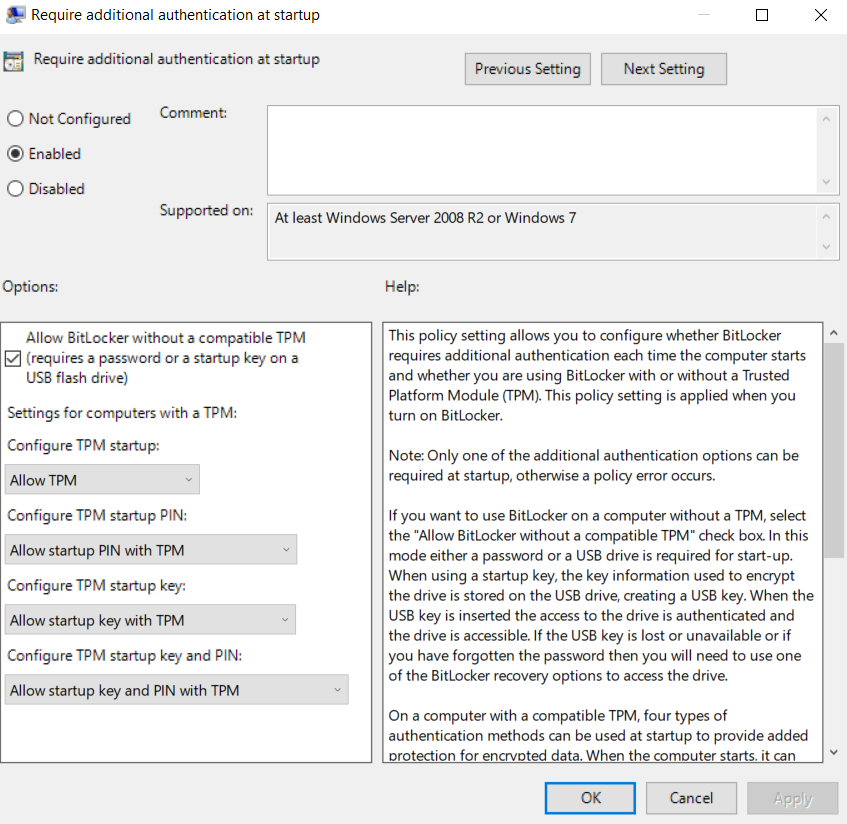
\includegraphics[width=0.7\linewidth]{../img/Encryption/computers-without-tpm.png}
    \caption{\acrshort{gpo} für BitLocker ohne \acrshort{tpm}}
\end{figure}
Zusätzlich kann nicht das Script verwendet werden, da vom Benutzer ein Passwort gesetzt werden muss.
Daher ist es am einfachsten, BitLocker für diese Geräte manuell zu aktivieren.
Dies geht auch mit Powershell ausgeführt als Administrator:
\begin{lstlisting}
    $Password = Read-Host -AsSecureString
    Add-BitLockerKeyProtector -MountPoint 'c:' -RecoveryPasswordProtector
    Enable-Bitlocker -MountPoint 'c:' -PasswordProtector -Password $Password
\end{lstlisting}
Die Festplatte wird beim nächsten Neustart verschlüsselt.


\subsubsection{Recovery Key auslesen}
Der Recovery Key ist auf den Computer Objekten in der Active Directory hinterlegt.
Dazu öffnet man die Einstellungen eines Computer Objektes und öffnet den Tab ``BitLocker Recovery'':
\begin{figure}[H]
    \centering
    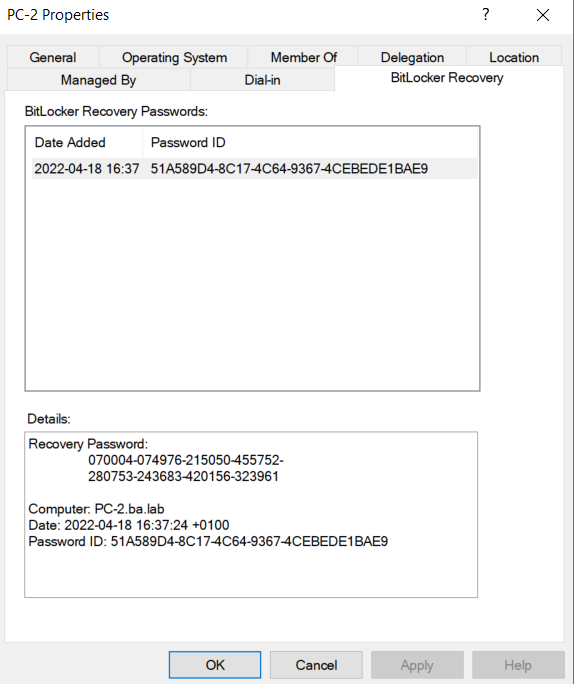
\includegraphics[width=0.7\linewidth]{../img/Encryption/bitlocker-recovery.png}
    \caption{Recovery Key für BitLocker}
\end{figure}
Dort findet man unter ``Recovery Password'' das Passwort um den Computer im Notfall zu entschlüsseln.